\makeatletter
\cxset{
 chapter opening=right,
 chapter toc=false,
 name=CHAPTER,
 numbering= WORDS, %WORDS gives errors
 number font-size=huge,
 number font-family=sffamily,
 number font-weight=bfseries,
 number before=\kern1em,
 number dot=,
 number after=,
 number position=rightname,
 % set chapter fonts 
 chapter font-family=sffamily,
 chapter font-weight=bfseries,
 chapter font-size=huge,
 chapter margin top=5cm,
 chapter margin left=0pt,
 chapter before=\par\hfill,
 chapter after=,
 chapter color=black,
 chapter spaceout=none,
 chapter title align=center,
 chapter afterindent=true,
 number color=black,
% chapter titles
 title margin top=30pt,
 title margin bottom=30pt,
 chapter title width=\textwidth,
 chapter title text-align=center,
 title font-family=sffamily,
 title font-color=black,
 title font-weight=bfseries,
 title font-size=huge,
 title font-shape=upshape,
 title before=,
 title after=,
% sections 
 section font-size=LARGE,
 section font-weight=normalfont,
 section font-family=sffamily,
 section color=black,
 section align=centering,
 section numbering=none,
 section indent=-1em,
 section beforeskip=20pt,
 section afterskip=10pt,
 section spaceout=soul,
 section font-shape=,
 pagestyle = plain,
 subsection color=black,
}

\chapter{Introduction to Style 10}

\addcontentsline{toc}{section}{Template 10 (style10)}

This style is very similar to the |verso chapter| style. I have reproduced it as close as possible to the book that gave me the inspiration titled \emph{Mind Machines}.

\begin{figure}[htb]
\centering
\fboxrule1pt
\fbox{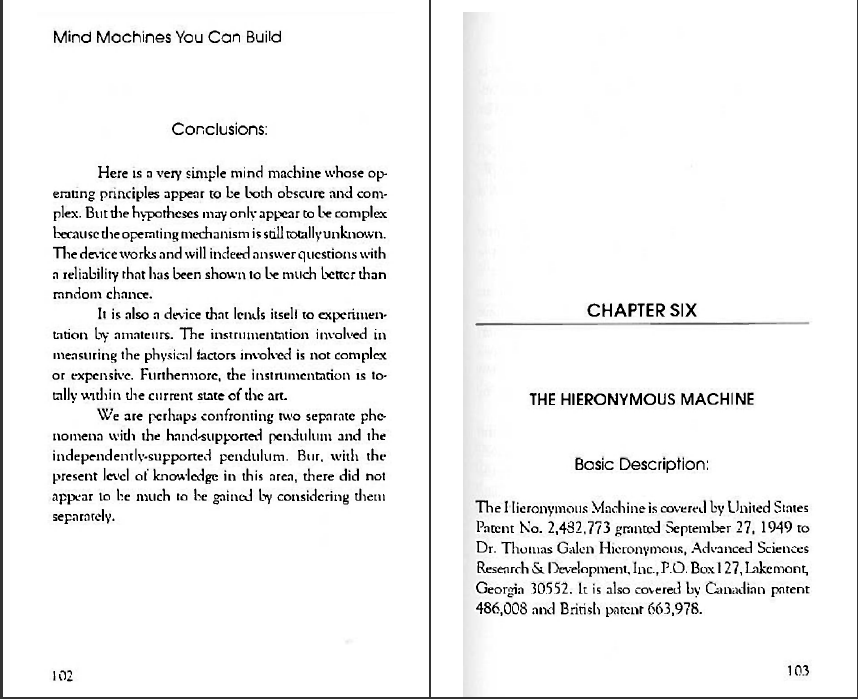
\includegraphics[width=0.8\textwidth]{./chapters/chapter10}}
\caption{Style ten example.}
\end{figure}

Another interesting aspect is that subsections are centered and have a colon at the end of the subsection title. The setting for this is the option \lstinline{numeric=WORDS}. Use either a capital for uppercase or \lstinline{numeric=words} for lowercase number labels.

\cxset{chapter toc=true,
          chapter margin top=0pt}
\makeatother
